\section*{Результаты измерений}

\subsection*{Исследование дифракции Френеля}

С помощью микрометрического винта была установлена ширина щели $0.30 \mm$. 
Ширина щели, измеренная микроскопом равна $0.3 \mm$. В ходе измерений было 
замечено, что у щели не ровные края. Неровность краев щели была видна, когда 
полностью закрытую щель освещали лампой, и она всё равно пропускала малую часть 
света. Данный дефект установки может оказать влияние на качество наблюдаемых 
дифракционных картин.

\begin{figure}[h]
	\begin{minipage}[h]{0.49 \linewidth}
		\centering
		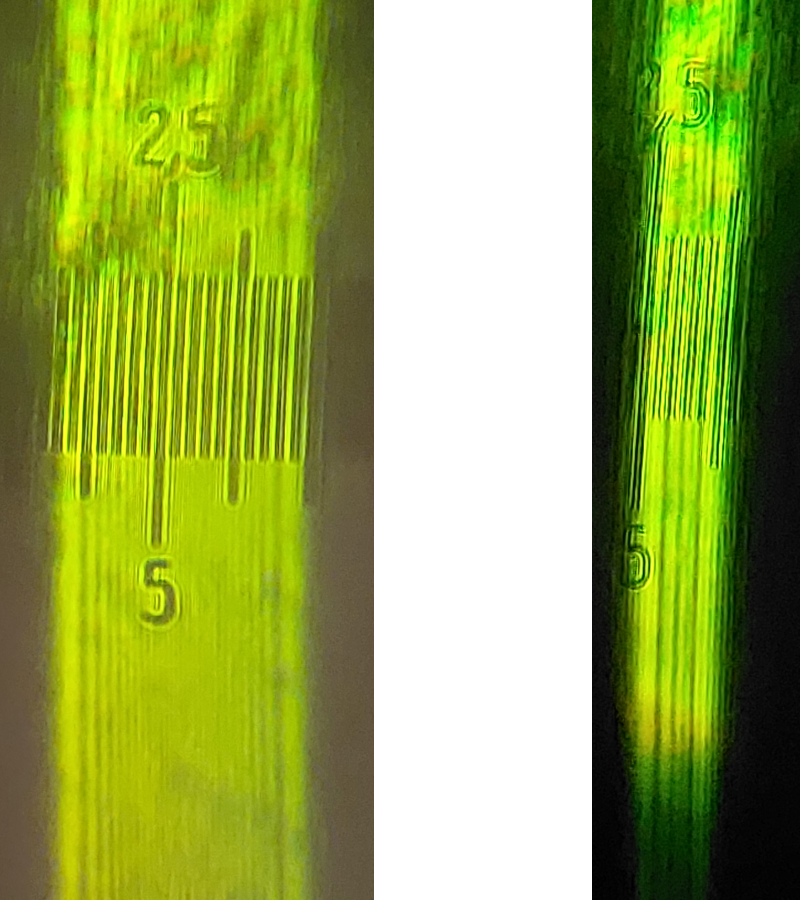
\includegraphics[width=0.8\linewidth]{../Изображения/Качественно Френель размер щели.png}
		\caption{}
		\label{img:Fresnel-diffraction-quality}
	\end{minipage}
	\hfill
	\begin{minipage}[h]{0.49 \linewidth}
		\centering
		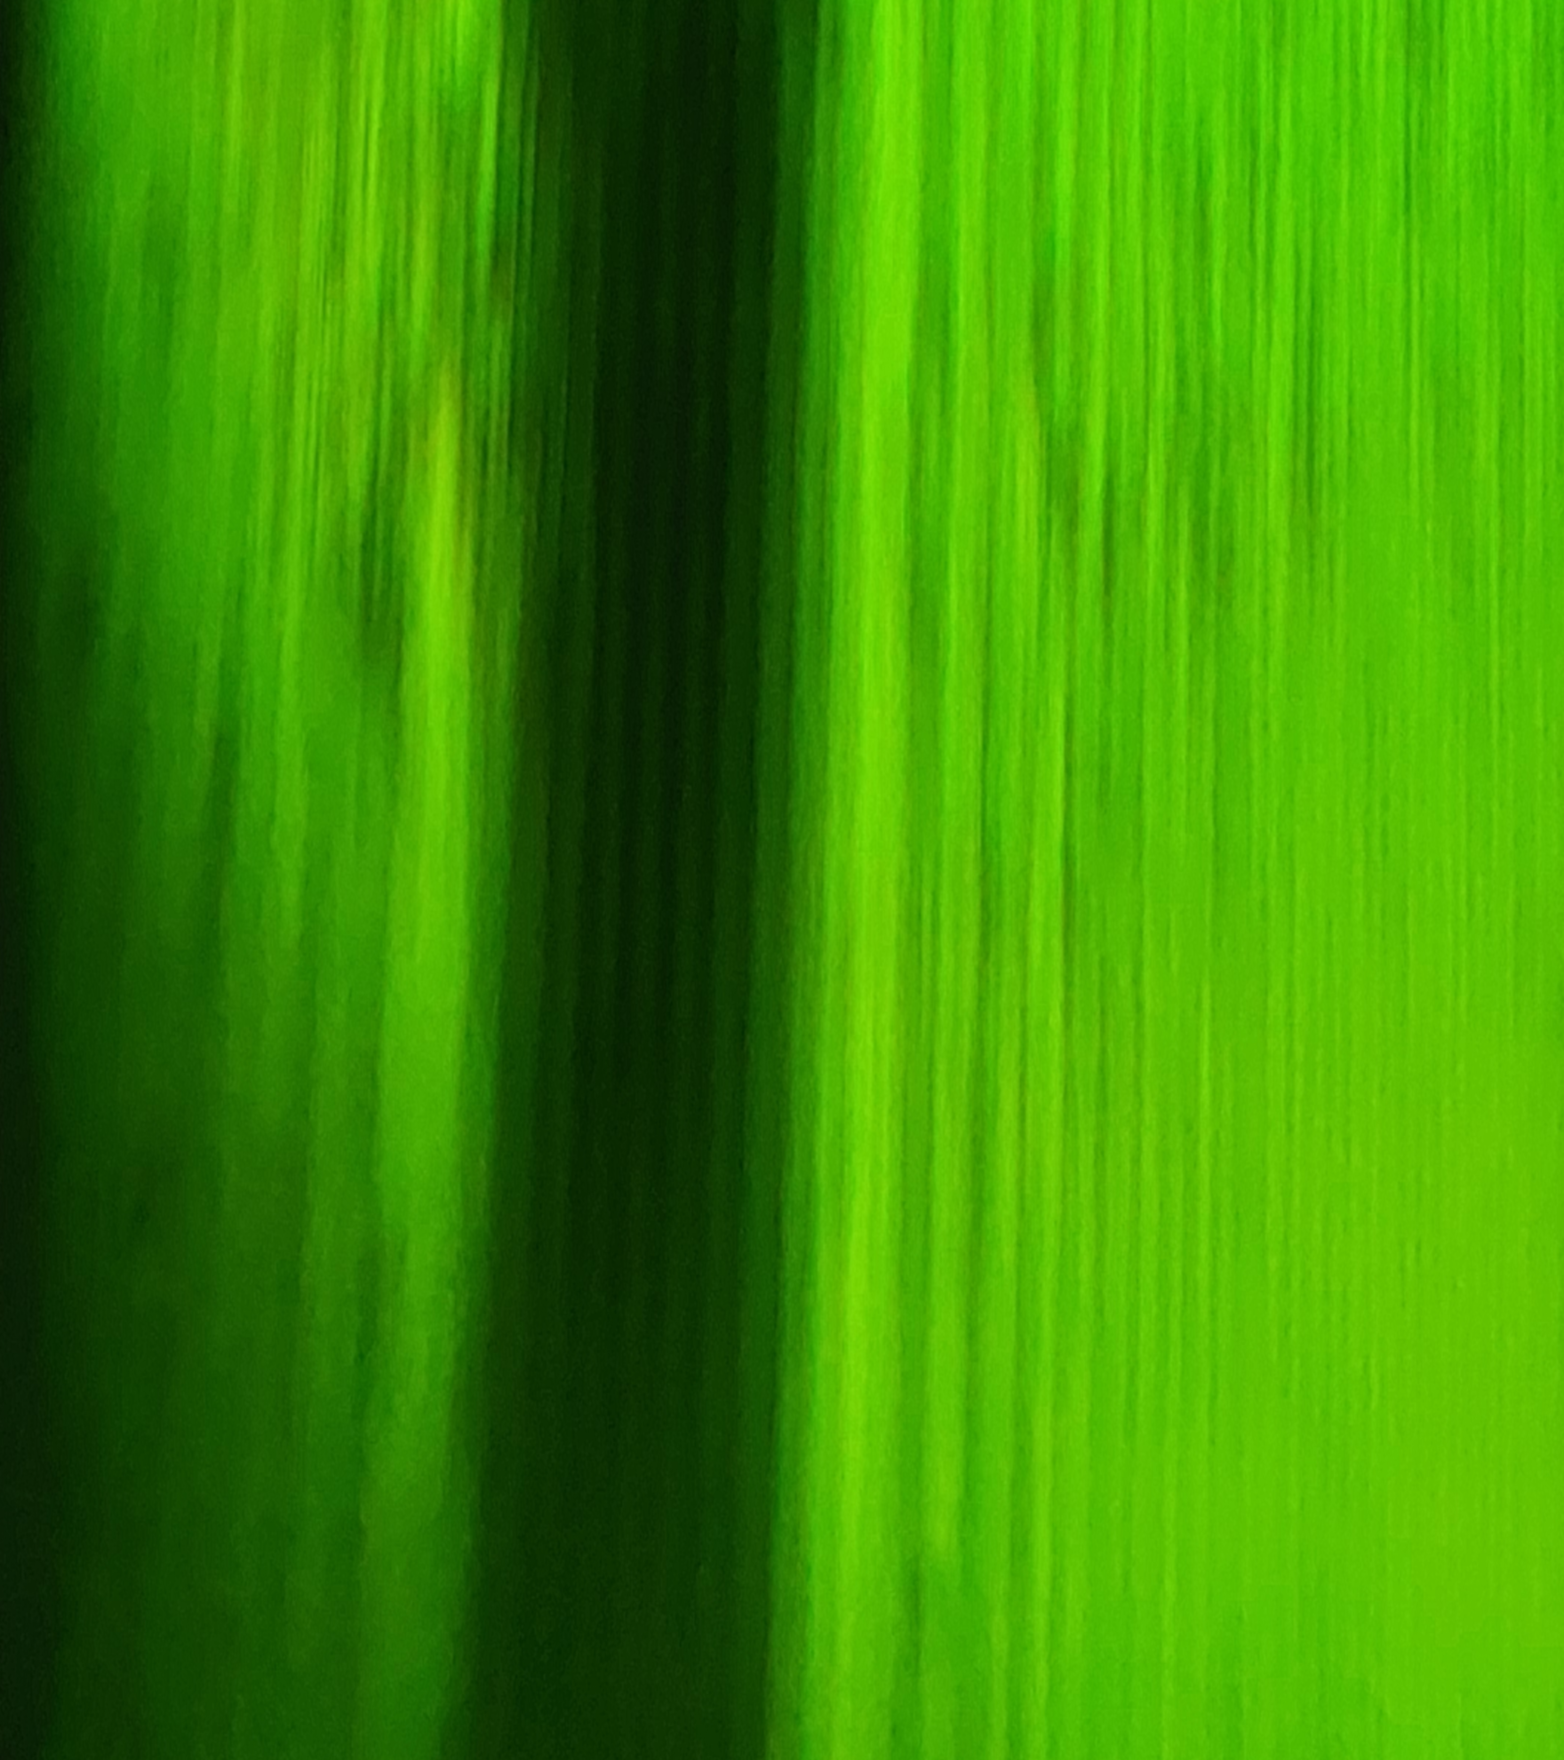
\includegraphics[width=0.8\linewidth]{../Изображения/Пятно Пуассона2.png}
		\caption{}
		\label{img:Poisson-spot}
	\end{minipage}
	\begin{tabular}{p{0.49\linewidth}p{0.49\linewidth}}
		Качественная зависимость дифракционной картины от ширины щели. Слева щель открыта больше, чем справа. Количество черных дифракционных слева больше, чем справа. &
		\centering
		Пятно Пуассона. \\
	\end{tabular}
\end{figure}

В ходе наблюдений было установлено (рис. 
$\ref{img:Fresnel-diffraction-quality}$), что при неизменном расстоянии до 
микроскопа, при увеличении размера щели, количество темных дифракционных полос 
увеличивается, они становятся более размытыми и меньшими по толщине.

В работе наблюдалась дифракция Френеля на препятствии (рис. 
$\ref{img:Poisson-spot}$). Из-за большого размера входной щели количество 
дифракционных полос большое, они размыты. Настроить установку для наблюдения 
более качественной картины не удалось, потому что при уменьшении размера 
входной щели, уменьшалась яркость картинки и дифракционные полосы были слабо 
различимы. Поэтому точное число тёмных дифракционных полос на фоне нити 
установить не удалось.

На рисунке изображена зависимость ширины открытых зон Шустера от их количества. 

\begin{figure}[h]
	\centering
	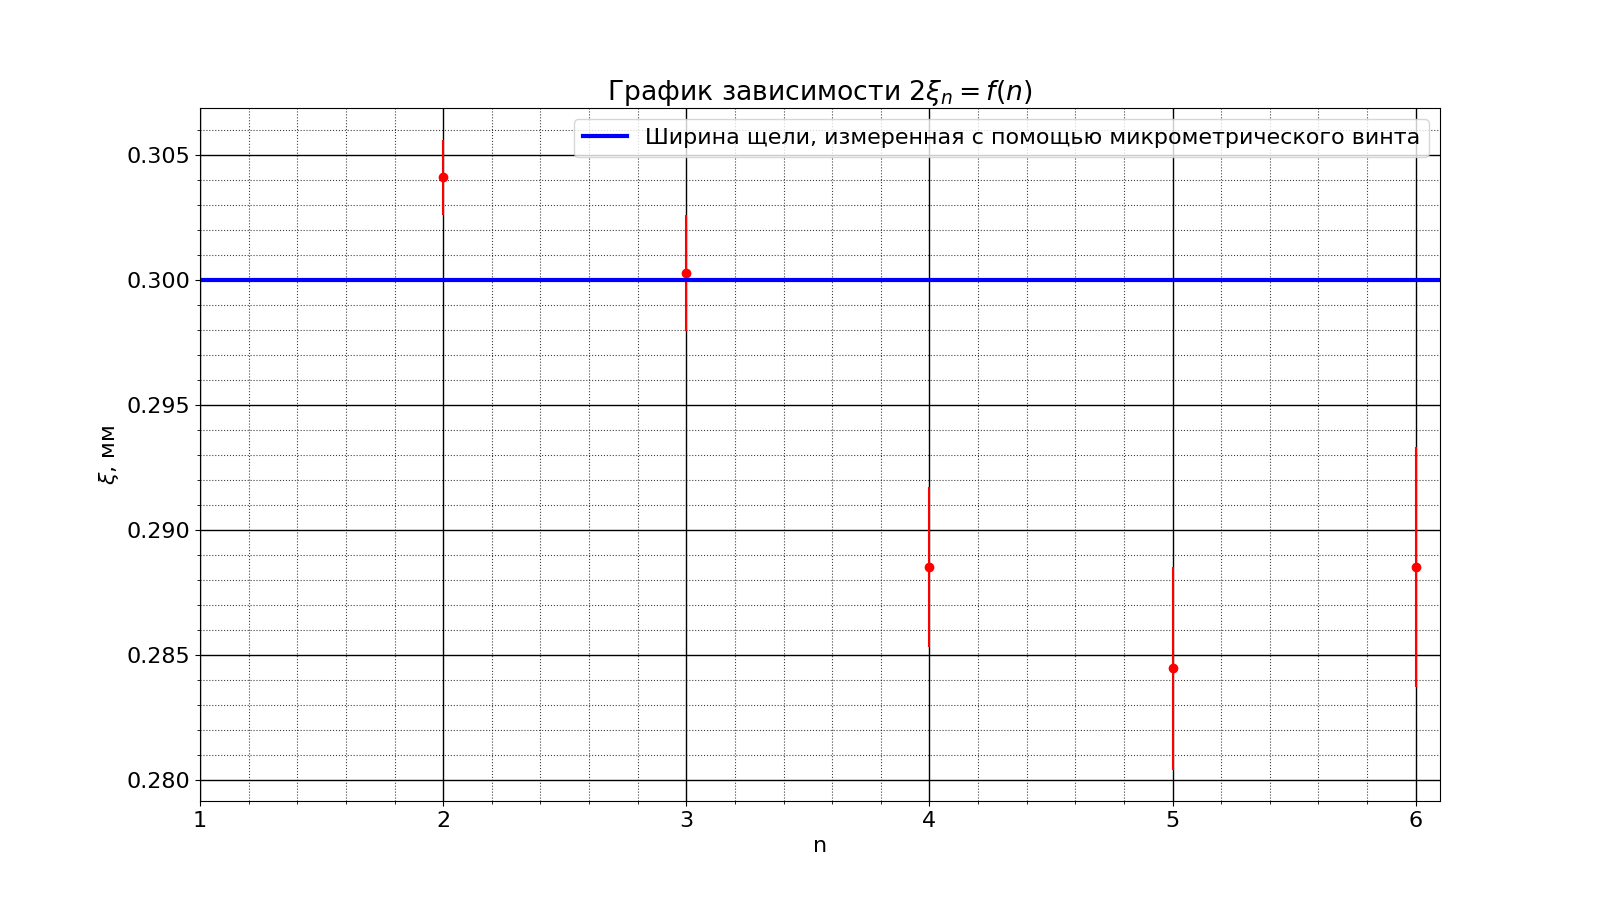
\includegraphics[width=0.88\textwidth]{../Изображения/xi_f(n).png}
	\caption{График зависимости ширины открытых зон Шустера от их количества}
\end{figure}

Дифракционная картина из $m$ полос наблюдается наиболее четко, когда открыто 
ровно $n = m + 1$ зона Френеля. Отклонения точек на графике от ширины щели 
связаны с 
тем, что расстояние до микроскопа устанавливалось так, чтобы дифракционная 
картина была наиболее резкой, данный критерий является субъективным и не 
является точным. Другая причина отклонения точек связана с погрешностью 
измерительной линейки, которая составляет $0.5 \mm$. Данная погрешность учтена 
на графике в виде крестов погрешности.

Так как зависимость $f(n)$ не является линейной, то оценим среднее значение 
ширины щели $2\bar\xi_n = 0.293 \pm 0.004 \mm$.

Итого были получены следующие значения ширины щели: \\
\begin{tabular}{|c|c|}
\hline
Микроскоп & 0.30 мм \\
\hline
Микрометрический винт & 0.30 мм \\
\hline
Средняя ширина открытых зон Шустера $2\bar\xi_n$ & $0.293 \pm 0.004$ мм \\
\hline
\end{tabular}

\subsection*{Исследование дифракции Фраунгофера}

В ходе наблюдений было установлено, что смещение щели $S_2$ в боковом 
направлении не приводит к сдвигу дифракционной картины.

На рисунке ниже изображен график зависимости расстояния от центра 
дифракционного минимума от его номера.

\begin{figure}[H]
	\centering
	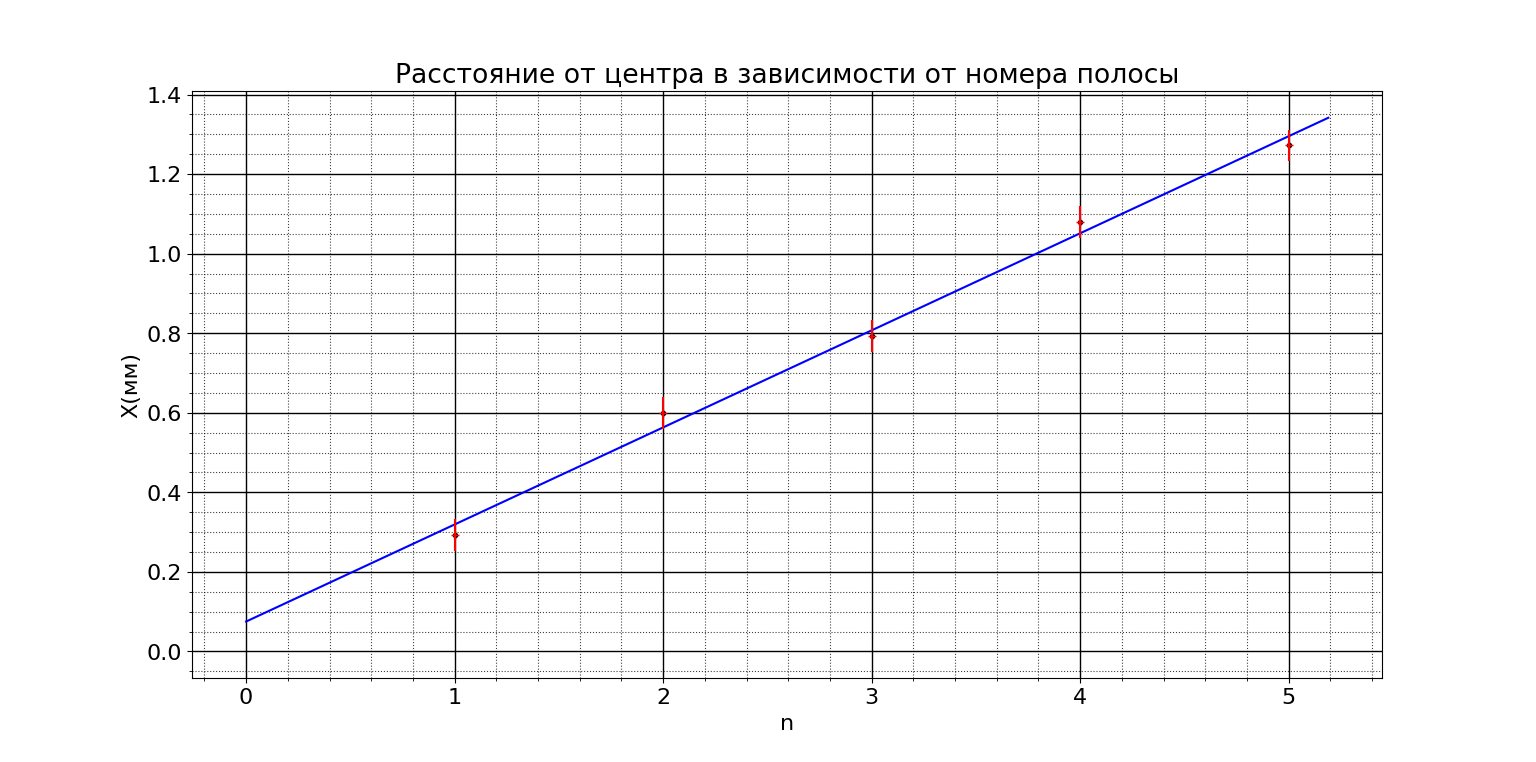
\includegraphics[width=0.88\textwidth]{../Изображения/X_n.png}
	\caption{График зависимости расстояния до дифракционного минимума от его 
	номера}
\end{figure}

Определим ширину щели $b$:
$$
x_m = m \frac{\lambda}{b} f_2
$$
где $x_m$ -- расстояние от центра дифракционной картины до $m$-ого минимума, 
$f_2$ -- фокусное расстояние собирающей линзы $Л_2$.

Измерения ширины щели при исследовании дифракции Фраунгофера:\\

\begin{tabular}{|c|c|}
	\hline
	Микроскоп & 0.30 мм \\
	\hline
	Микрометр & 0.18 мм \\
	\hline
	Дифракция Фраунгофера & 0.41 $\pm$ 0.06 мм \\
	\hline
\end{tabular}

Результаты сильно расходятся, скорее всего, из-за ошибки, допущенной в ходе 
выполнения работы. Установить точную причину расхождения результатов не удалось.